\documentclass{article}

\usepackage[utf8]{inputenc}
\usepackage[brazil]{babel}

\title{Exercício 2: Gaussiana no Espaço $R^n$}
\author{Rúbia Reis Guerra \\ 2013031143}

\usepackage{Sweave}
\begin{document}
\Sconcordance{concordance:gaussrn.tex:gaussrn.Rnw:%
1 8 1 1 0 7 1 1 2 1 0 2 1 1 6 5 0 1 2 1 0 1 4 2 0 2 1 3 0 1 2 1 1 1 4 3 %
0 5 1 1 4 2 0 1 4 2 0 1 1 1 4 2 0 1 1 1 4 2 0 1 1 1 4 2 0 1 1 3 0 1 2 2 %
1 1 2 5 0 1 2 1 1 1 4 3 0 1 1 1 8 7 0 1 3 1 0 1 1 8 0 1 3 7 0 1 2 1 1 1 %
4 3 0 1 1 1 8 7 0 1 3 1 0 1 1 8 0 1 3 7 0 1 2 1 1 1 4 3 0 1 43 42 0 1 4 %
7 0 1 1 6 0 1 2 1 1}

\maketitle

\section{Classificador Bayesiano: Gaussiana no Espaço $R^n$}
Nesta atividade, foi proposta a amostragem de dados do dataset Iris, seguida da divisão em conjuntos de teste e treino e classifiação bayesiana.

\subsection{Funções e Parâmetros}
\begin{Schunk}
\begin{Sinput}
> library('plot3D')
> library('MASS')
> rm(list=ls())
> ###########################
> # Funções #
> # Densidade de probabilidade multivariada #
> pdfnvar <- function(x,m,k,V){
+   ((1/(sqrt(((2*pi)^k)*det(V))))
+    *exp(-0.5*(t(x-m) %*% solve(V) %*% (x-m))))}
> # Classificação Bayesiana #
> class <- function(pxc1,pxc2,pc1,pc2){ifelse(((pxc1/pxc2) >= (pc2/pc1)), 1, 2)}
> ###########################
> # Parâmetros #
> nc1 <- 100
> nc2 <- 50
> rep <- 30
\end{Sinput}
\end{Schunk}

\subsection{Particionamento do Dataset Iris}
\begin{Schunk}
\begin{Sinput}
> ###########################
> # Dataset Iris #
> data(iris)
> X <- as.matrix(iris[,1:4])
> Y <- as.matrix(iris[,5])
> Y1 <- matrix(1, nrow=nc1,ncol=1)
> Y2 <- matrix(2, nrow=nc2,ncol=1)
> Y <- rbind(Y1,Y2)
> ###########################
> # Amostrar dados #
> index <- sample(2, nrow(iris), replace=TRUE, prob=c(0.70,0.30))
> ###########################
> # Conjunto de treinamento #
> training <- X[index==1,1:4]
> trainingLabels <- Y[index==1]
> ###########################
> # Conjunto de teste #
> test <- X[index==2, 1:4]
> testLabels <- Y[index==2]
> ###########################
> # Índices das classes c1, c2 #
> i1 <- which(trainingLabels==1)
> i2 <- which(trainingLabels==2)
> ###########################
> # Probabilidades a priori #
> pc1 <- nc1/(nc1+nc2)
> pc2 <- nc2/(nc1+nc2)
\end{Sinput}
\end{Schunk}

\subsection{Análise: Dataset Iris}
A partir da análise dos gráficos de dispersão do dataset Iris, observa-se a sobreposição das espécies 2 e 3 (\textit{virginica} e \textit{versicolor}, cores vermelha e verde), em contraste com a separabilidade da espécie 1 (\textit{setosa}, cor preta). Portanto, no momento da rotulação das classes 1 e 2 utilizadas nesta atividade, caso a classe 1 corresponda à espécie \textit{setosa} e a classe 2, \textit{virginica} e \textit{versicolor}, espera-se que o classificador bayesiano resulte em 100\% de acertos para o grupo de treinamento. Caso contrário, rotulando as espécies \textit{setosa} e \textit{virginica} como classe 1, e \textit{versicolor} como classe 2, considerando que as espécies 2 e 3 apresentam alguma sobreposição, espera-se que o classificador retorne uma parcela de exemplos rotulados erroneamente. 
\begin{Schunk}
\begin{Sinput}
> pairs(Species~., data=iris, main='Dataset Iris', col=iris$Species)
\end{Sinput}
\end{Schunk}
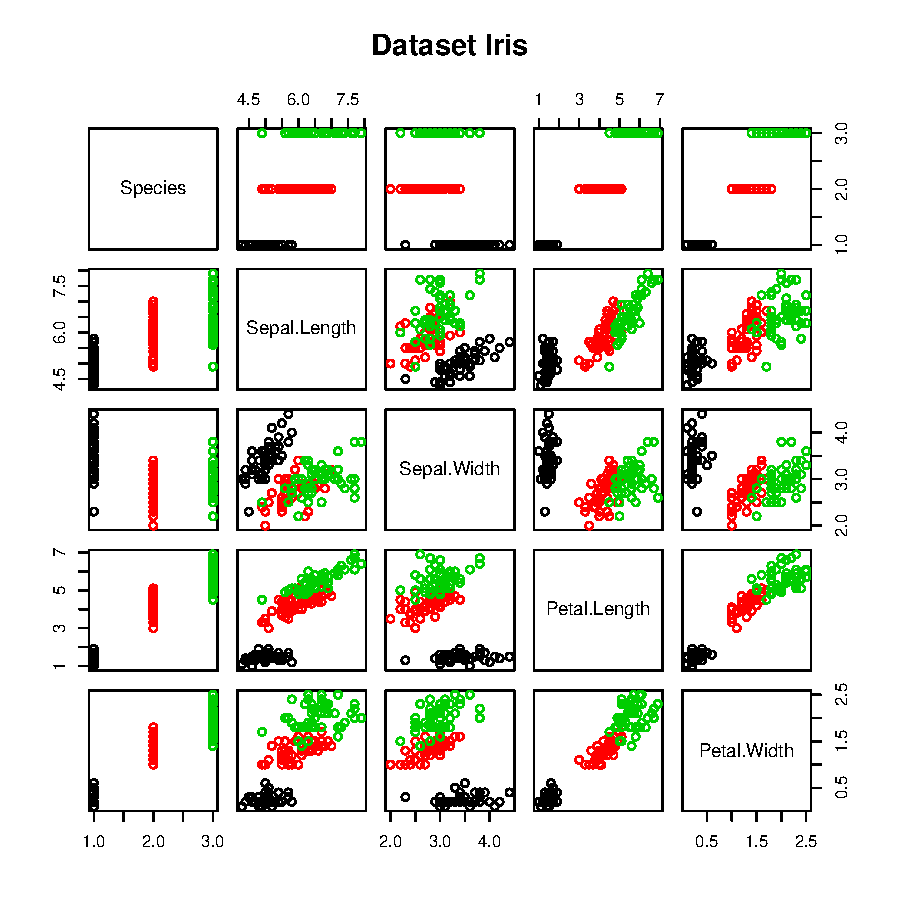
\includegraphics{gaussrn-003}

\subsection{Classificação: Conjunto de Treinamento}
\begin{Schunk}
\begin{Sinput}
> ###########################
> # Verossimilhança e classificação: conjunto de treinamento #
> trainingY <- c()
> ntr <- dim(training)[1]
> for (i in 1:ntr)
+ {
+   pxc1 <- pdfnvar(training[i,1:4],colMeans(training[i1,1:4]),
+                   (dim(training)[2]),cov(training[i1,1:4]))
+   pxc2 <- pdfnvar(training[i,1:4],colMeans(training[i2,1:4]),
+                   (dim(training)[2]),cov(training[i2,1:4]))
+   trainingY[i] <- ifelse(((pxc1/pxc2) >= (pc2/pc1)), 1, 2)
+ }
> # Matriz de confusão #
> trainingCM <- table(trainingY,trainingLabels)
> trainingCM
\end{Sinput}
\begin{Soutput}
         trainingLabels
trainingY  1  2
        1 79  2
        2  1 34
\end{Soutput}
\begin{Sinput}
> # Acertos #
> paste(formatC((((trainingCM[1,1]+trainingCM[2,2])/dim(training)[1])*100),digits=4), "%", sep="")
\end{Sinput}
\begin{Soutput}
[1] "97.41%"
\end{Soutput}
\end{Schunk}

\subsection{Classificação: Conjunto de Teste}
\begin{Schunk}
\begin{Sinput}
> ###########################
> # Verossimilhança e classificação: conjunto de teste #
> testY <- c()
> nte <- dim(test)[1]
> for (i in 1:nte)
+ {
+   pxc1 <- pdfnvar(test[i,1:4],colMeans(training[i1,1:4]),
+                   (dim(training)[2]),cov(training[i1,1:4]))
+   pxc2 <- pdfnvar(test[i,1:4],colMeans(training[i2,1:4]),
+                   (dim(training)[2]),cov(training[i2,1:4]))
+   testY[i] <- ifelse(((pxc1/pxc2) >= (pc2/pc1)), 1, 2)
+ }
> # Matriz de confusão #
> testCM <- table(testY,testLabels)
> testCM
\end{Sinput}
\begin{Soutput}
     testLabels
testY  1  2
    1 20  1
    2  0 13
\end{Soutput}
\begin{Sinput}
> # Acertos #
> paste(formatC((((testCM[1,1]+testCM[2,2])/dim(test)[1])*100),digits=4), "%", sep="")
\end{Sinput}
\begin{Soutput}
[1] "97.06%"
\end{Soutput}
\end{Schunk}

\subsection{Classificação: Conjunto de Teste ($n$ Treinos)}
\begin{Schunk}
\begin{Sinput}
> ###########################
> # Classificação (para n repetições) #
> acc <- c() # acertos por treino
> for(j in 1:rep){
+   ###########################
+   # Misturar dados #
+   index <- sample(2, nrow(iris), replace=TRUE, prob=c(0.70,0.30))
+   
+   ###########################
+   # Conjunto de treinamento #
+   training <- X[index==1,1:4]
+   trainingLabels <- Y[index==1]
+   
+   ###########################
+   # Conjunto de teste #
+   test <- X[index==2, 1:4]
+   testLabels <- Y[index==2]
+   
+   ###########################
+   # Classificação #
+   # Índices das classes c1, c2 #
+   i1 <- which(trainingLabels==1)
+   i2 <- which(trainingLabels==2)
+   
+   # Probabilidade a priori #
+   pc1 <- nc1/(nc1+nc2)
+   pc2 <- nc2/(nc1+nc2)
+   
+   # Verossimilhança e classificação: Conjunto de teste #
+   testY <- c()
+   nte <- dim(test)[1]
+   for (i in 1:nte)
+   {
+     pxc1 <- pdfnvar(test[i,1:4],colMeans(training[i1,1:4]),
+                     (dim(training)[2]),cov(training[i1,1:4]))
+     pxc2 <- pdfnvar(test[i,1:4],colMeans(training[i2,1:4]),
+                     (dim(training)[2]),cov(training[i2,1:4]))
+     testY[i] <- ifelse(((pxc1/pxc2) >= (pc2/pc1)), 1, 2)
+   }
+   
+   # Matriz de confusão #
+   testCM <- table(testY,testLabels)
+   
+   # Acertos #
+   acc[j] <- (testCM[1,1]+testCM[2,2])/(dim(test)[1])
+ }
> ###########################
> # Média e desvio padrão dos acertos #
> paste(formatC((mean(acc)*100),digits=4), "%", sep="")
\end{Sinput}
\begin{Soutput}
[1] " 95.6%"
\end{Soutput}
\begin{Sinput}
> paste(formatC((sd(acc)*100),digits=3), "%", sep="")
\end{Sinput}
\begin{Soutput}
[1] "3.18%"
\end{Soutput}
\end{Schunk}

\end{document}
